\documentclass[11pt,a4paper]{article}

\usepackage[utf8]{inputenc}
\usepackage[T1]{fontenc}
\usepackage{lmodern}
\usepackage[margin=0.85in]{geometry}
\usepackage{graphicx}
\usepackage{xcolor}
\usepackage{booktabs}
\usepackage{array}
\usepackage{multirow}
\usepackage{amsmath,amssymb}
\usepackage{enumitem}
\usepackage{tcolorbox}
\tcbuselibrary{skins,breakable}
\usepackage{hyperref}
\usepackage{caption}
\usepackage{subcaption}
\usepackage{fancyhdr}
\usepackage{titlesec}

% Color Palette
\definecolor{primaryblue}{HTML}{1E3A8A}
\definecolor{accentblue}{HTML}{2563EB}
\definecolor{softblue}{HTML}{EFF6FF}
\definecolor{borderblue}{HTML}{BFDBFE}
\definecolor{tealbox}{HTML}{F0FDFA}
\definecolor{tealborder}{HTML}{5EEAD4}
\definecolor{amberbox}{HTML}{FFFBEB}
\definecolor{amberborder}{HTML}{FCD34D}
\definecolor{darkgray}{HTML}{1F2937}
\definecolor{mutedgray}{HTML}{4B5563}

\hypersetup{
    colorlinks=true,
    linkcolor=primaryblue,
    urlcolor=accentblue,
    citecolor=primaryblue,
    pdftitle={ECRformer-Lite and Structural Sharpening: Project Briefing},
    pdfauthor={Vaishnav}
}

% Section Formatting
\titleformat{\section}
  {\Large\bfseries\color{primaryblue}}
  {\thesection.}{0.6em}{}[\titlerule]
\titleformat{\subsection}
  {\large\bfseries\color{darkgray}}
  {\thesubsection}{0.5em}{}

% Header / Footer
\pagestyle{fancy}
\fancyhf{}
\fancyhead[L]{\small\textcolor{mutedgray}{\textbf{Project Briefing:} SAR-Guided Satellite Cloud Removal (ECRformer-Lite)}}
\fancyhead[R]{\small\textcolor{mutedgray}{\href{https://github.com/yovyshh/ecrformer}{github.com/yovyshh/ecrformer}}}
\fancyfoot[C]{\small\textcolor{mutedgray}{Page \thepage}}
\renewcommand{\headrulewidth}{0.4pt}

% Custom Boxes
\newtcolorbox{laymanbox}[1]{
  enhanced,
  breakable,
  colback=softblue,
  colframe=accentblue,
  coltitle=white,
  fonttitle=\bfseries,
  title={#1},
  arc=3mm,
  boxrule=1pt,
  left=3mm, right=3mm, top=2.5mm, bottom=2.5mm
}

\newtcolorbox{contribbox}[1]{
  enhanced,
  breakable,
  colback=tealbox,
  colframe=tealborder!80!black,
  coltitle=white,
  fonttitle=\bfseries,
  title={#1},
  arc=3mm,
  boxrule=1pt,
  left=3mm, right=3mm, top=2.5mm, bottom=2.5mm
}

\newtcolorbox{hardwarebox}[1]{
  enhanced,
  breakable,
  colback=amberbox,
  colframe=amberborder!85!black,
  coltitle=darkgray,
  fonttitle=\bfseries,
  title={#1},
  arc=3mm,
  boxrule=1pt,
  left=3mm, right=3mm, top=2.5mm, bottom=2.5mm
}

\setlength{\parskip}{0.45em}
\setlength{\parindent}{0pt}

\begin{document}

% ============================================================================
% TITLE BANNER
% ============================================================================
\begin{center}
    {\LARGE\bfseries\color{primaryblue} SAR-Guided Optical Satellite Cloud Removal via ECRformer-Lite, Soft-Mask Blending, and Multi-Stage Structural Sharpening}\\[0.8em]
    {\large\textbf{Executive Research Briefing \& System Architecture Overview}}\\[0.5em]
    {\normalsize \textbf{Author:} Vaishnav \quad|\quad \textbf{Code \& Documentation:} \href{https://github.com/yovyshh/ecrformer}{\texttt{https://github.com/yovyshh/ecrformer}}}
\end{center}

\vspace{0.3em}

\begin{laymanbox}{At a Glance: What Did We Build? (In Simple Terms)}
Optical satellites (like Europe's Sentinel-2) take high-resolution color photographs of the Earth to monitor crops, forests, floods, and cities. However, \textbf{more than 50\% of the Earth's surface is covered by clouds at any given moment}, turning satellite photos into blank white sheets.

We built and trained a lightweight, deep-learning AI system (\textbf{3.62 million parameters}) that acts like ``digital X-ray vision'' for satellite imagery:
\begin{enumerate}[leftmargin=1.5em, itemsep=2pt, topsep=2pt]
    \item \textbf{Seeing Through Clouds with Radar:} It combines a \textbf{Cloudy Optical Image} (Sentinel-2) with a \textbf{Cloud-Penetrating Radar Image} (Sentinel-1 SAR) taken over the same area.
    \item \textbf{Keeping Clear Areas 100\% Intact:} It uses a refined \textbf{Soft Cloud Mask} so that any ground already visible in the original photo is kept untouched, while only cloudy regions are reconstructed.
    \item \textbf{Restoring Crisp Roads \& Field Edges:} Standard AI cloud-removal models produce blurry, smudged patches under thick clouds. We designed a custom \textbf{Multi-Stage Sharpening Pipeline} (combining scale-decoupled color supervision, edge gradients, perceptual features, and a high-frequency adversarial discriminator) that boosts fine spatial detail retention from \textbf{$\sim$40\% to over 90\%} while maintaining \textbf{$\sim$30--33 dB PSNR}.
\end{enumerate}
\end{laymanbox}

% ============================================================================
% SECTION 1: THE PROBLEM STATEMENT
% ============================================================================
\section{The Problem: Why Satellite Cloud Removal is Hard}

\subsection{1.1 The Cloud Blindness Problem in Optical Satellites}
Optical satellites (\textbf{Sentinel-2}) capture sunlight reflected off the Earth across visible colors (Red, Green, Blue) and Near-Infrared (NIR, which measures plant health). Because sunlight cannot pass through thick water droplets, clouds completely block the camera's view:
\begin{itemize}[leftmargin=1.5em, itemsep=2pt]
    \item \textbf{Thin Haze:} Partially dims and washes out ground colors, reducing contrast.
    \item \textbf{Thick / Opaque Clouds:} Completely erase 100\% of the ground information underneath. You cannot simply ``adjust brightness or contrast'' to recover what is hidden under an opaque cloud---the ground pixels are physically missing.
\end{itemize}

\subsection{1.2 How Radar (SAR) Helps---And Why It Is Not Enough Alone}
Unlike optical cameras, \textbf{Synthetic Aperture Radar (Sentinel-1 SAR)} sends out microwave radio pulses (\texttt{C-band}, $\sim 5.6\text{ cm}$ wavelength) that pass right through clouds, smoke, and rain, day or night.
\begin{itemize}[leftmargin=1.5em, itemsep=2pt]
    \item \textbf{What Radar Sees:} Physical geometry and surface roughness---roads, rivers, building corners, mountain ridges, and agricultural field boundaries.
    \item \textbf{What Radar Cannot See:} Color or vegetation chlorophyll. Furthermore, radar images look grainy to the human eye because of wave interference (\textit{radar speckle noise}).
    \item \textbf{The Core AI Task:} Fuse the \textbf{structural geometry from Radar (Sentinel-1)} with the \textbf{color context from Optical (Sentinel-2)} to paint back sharp, accurate, cloud-free optical imagery.
\end{itemize}

\subsection{1.3 The Two Major Flaws in Existing Baselines}
When we first trained the baseline \textbf{ECRformer-Lite} model, it achieved a good pixel-accuracy score (\textbf{30.20 dB PSNR}), but visual inspection revealed two serious real-world problems:
\begin{enumerate}[leftmargin=1.5em, itemsep=2pt]
    \item \textbf{The ``Blurriness Trap'' Under Thick Clouds:} Standard AI models are trained with pixel-averaging losses ($L_1$ and SSIM). When a cloud completely hides a farm, the model is uncertain whether a road edge is at pixel 50 or pixel 51. To minimize penalty, the AI guesses the \textbf{average of all possibilities}, creating a blurry, washed-out smudge that loses over \textbf{55\% to 65\%} of fine surface details.
    \item \textbf{Damage to Cloud-Free Pixels \& Boundary Seams:} If the AI replaces the entire image, it slightly degrades pixels that had \textit{no clouds at all}. Conversely, if you paste the AI prediction using a raw binary cloud mask, any tiny error or pinhole in the cloud mask leaves ugly ``cut-and-paste'' seams around cloud borders.
\end{enumerate}

% ============================================================================
% SECTION 2: THE DATASET
% ============================================================================
\section{The Dataset: SEN12MS-CR (Multimodal Satellite Triplets)}

We train and evaluate our system on the benchmark \textbf{SEN12MS-CR} dataset, which contains globally distributed, co-registered satellite image patches aligned to a $10\text{m}\times 10\text{m}$ ground resolution per pixel ($256 \times 256$ pixels per patch $= 2.56\text{ km} \times 2.56\text{ km}$ on the ground).

\begin{table}[h!]
\centering
\small
\renewcommand{\arraystretch}{1.25}
\begin{tabular}{p{3.2cm} p{2.5cm} p{3.2cm} p{5.5cm}}
\toprule
\textbf{Data Modality} & \textbf{Channels Used} & \textbf{Normalization Range} & \textbf{What It Tells the AI (Layman Role)} \\
\midrule
\textbf{1. Cloudy Optical} \newline (Sentinel-2 L1C) & \textbf{4 Bands:} \newline B04 (Red), B03 (Green), B02 (Blue), B08 (NIR) & Reflectance clipped to $[0, 10000] \rightarrow [0, 1]$ & Provides true colors and sharp ground details in clear areas; shows where haze/clouds obscure the view. \\
\addlinespace[2pt]
\textbf{2. Radar (SAR)} \newline (Sentinel-1 GRD) & \textbf{2 Channels:} \newline VV \& VH Polarizations & Backscatter dB clipped:\newline VV: $[-25, 0] \rightarrow [0, 1]$\newline VH: $[-32.5, 0] \rightarrow [0, 1]$ & Penetrates 100\% of clouds. Gives the physical outline of roads, rivers, buildings, and crop boundaries. \\
\addlinespace[2pt]
\textbf{3. Cloud Mask} \newline (Derived Input) & \textbf{1 Channel:} \newline Soft Probability $M \in [0,1]$ & Continuous $[0, 1]$ \newline ($0=$ Clear, $1=$ Opaque) & Tells the network \textit{where} to trust the optical input ($M \approx 0$) vs.\ where to reconstruct from radar ($M \approx 1$). \\
\midrule
\textbf{Combined Input} & \textbf{7 Channels Total} & Tensor: $[B, 7, 256, 256]$ & Fed into the dual-stream ECRformer-Lite generator. \\
\addlinespace[2pt]
\textbf{Target Ground Truth} & \textbf{4 Bands} (Cloud-Free S2) & Tensor: $[B, 4, 256, 256]$ & Cloud-free Sentinel-2 image acquired over the exact same location within a short temporal window. \\
\bottomrule
\end{tabular}
\caption{Summary of the 7-channel multimodal input and 4-channel optical target from SEN12MS-CR.}
\end{table}

% ============================================================================
% SECTION 3: HARDWARE LIMITATIONS & ENGINEERING CHALLENGES
% ============================================================================
\section{Hardware Limitations \& Practical Engineering Challenges}

A crucial constraint of this research was executing the entire multi-stage training, ablation, and sharpening pipeline on a \textbf{single personal GPU} under strict memory (VRAM) and compute limits, rather than a multi-node university supercomputer cluster.

\begin{hardwarebox}{How We Overcame Single-GPU Hardware Constraints (30+ Hours of Training)}
\begin{itemize}[leftmargin=1.5em, itemsep=3pt, topsep=2pt]
    \item \textbf{Memory Wall of Standard Transformers:} Standard Vision Transformers compute pixel-to-pixel attention across all $256 \times 256 = 65,536$ pixels, requiring a $65,536 \times 65,536$ matrix ($\sim 16\text{ GB}$ per layer), which immediately crashes a consumer GPU with an Out-Of-Memory (OOM) error.
    \item \textbf{Lightweight Architecture Design (\texttt{ECRformer-Lite}):} We replaced spatial $H\times W$ attention with \textbf{Transposed Channel Attention (MDTA)}, which computes a compact $C \times C$ spectral covariance matrix ($64\times 64$ or $128\times 128$). This reduced the total generator size to just \textbf{3,619,070 parameters ($\sim 3.62\text{M}$)} while preserving global context.
    \item \textbf{Gradient Accumulation \& Mixed Precision (AMP FP16):} Training with VGG-16 perceptual features, a PatchGAN discriminator, and $256 \times 256$ 7-channel tensors simultaneously pushed VRAM to its physical ceiling. We used \textbf{physical batch size $= 1$} combined with \textbf{8-step Gradient Accumulation} (simulating an effective batch size of 8) and PyTorch Automatic Mixed Precision (\texttt{fp16}).
    \item \textbf{Fast Tensor Pre-Caching:} Reading raw GeoTIFF satellite tiles from disk during training caused severe I/O bottlenecks. We pre-converted the training and validation splits into compressed \texttt{.pt} tensor caches, enabling over \textbf{30+ hours of continuous local GPU training} across four progressive optimization stages.
\end{itemize}
\end{hardwarebox}

% ============================================================================
% SECTION 4: FOUNDATIONAL PAPERS & LITERATURE BASIS
% ============================================================================
\section{Foundational Papers \& Research Lineage}

Our implementation synthesizes concepts from five core peer-reviewed works in remote sensing and computer vision, adapting them for sharp multimodal cloud removal under single-GPU constraints:

\begin{enumerate}[leftmargin=1.6em, itemsep=4pt]
    \item \textbf{Multimodal SAR-Optical Dataset \& Benchmark:} \textit{Ebel et al.\ (IEEE TGRS, 2020)}, ``SEN12MS-CR: A curated dataset of georeferenced multi-spectral Sentinel-1/2 imagery for deep learning and data fusion.'' Establishes the physics of pairing C-band SAR with multispectral Sentinel-2 imagery.
    \item \textbf{Dual-Stream SAR-Optical Cloud Removal (ECRformer / GLF-CR):} \textit{Xu et al.\ (IEEE TGRS, 2022)} and recent Dual-Stream Cloud Removal Transformers. Establishes separate encoders for optical and SAR streams followed by cross-modal fusion so radar speckle noise does not corrupt optical colors early in the network.
    \item \textbf{Linear-Complexity Channel Attention (Restormer):} \textit{Zamir et al.\ (CVPR, 2022)}, ``Restormer: Efficient Transformer for High-Resolution Image Restoration.'' Provides the Multi-Dconv Head Transposed Attention (\textbf{MDTA}) and Gated-Dconv Feed-Forward Network (\textbf{GDFN}) used in our bottleneck.
    \item \textbf{Frequency-Domain Reconstruction (Focal Frequency Loss / SDFL):} \textit{Jiang et al.\ (ICCV, 2021)}. Inspires our \textbf{Spatial-Spectral Dual-Domain Frequency Loss (SDFL)}, which applies a 2D Fast Fourier Transform (FFT) during training to supervise high-frequency amplitude and phase alignment.
    \item \textbf{Conditional PatchGAN \& Perceptual Supervision:} \textit{Isola et al.\ (CVPR, 2017, Pix2Pix)}, \textit{Miyato et al.\ (ICLR, 2018, Spectral Normalization)}, and \textit{Johnson et al.\ (ECCV, 2016, Perceptual Losses)}. Adapted into our \textbf{11-Channel High-Pass Conditional PatchGAN} and dual-triplet VGG-16 feature matching to eliminate regression-to-the-mean blurring.
\end{enumerate}

% ============================================================================
% SECTION 5: PROPOSED PIPELINE & ARCHITECTURE
% ============================================================================
\newpage
\section{Proposed System Architecture \& 4-Stage Pipeline}

Figure \ref{fig:pipeline} illustrates the complete end-to-end architecture of our system, from raw satellite inputs to the final sharpened, mask-blended optical reconstruction.

\begin{figure}[h!]
    \centering
    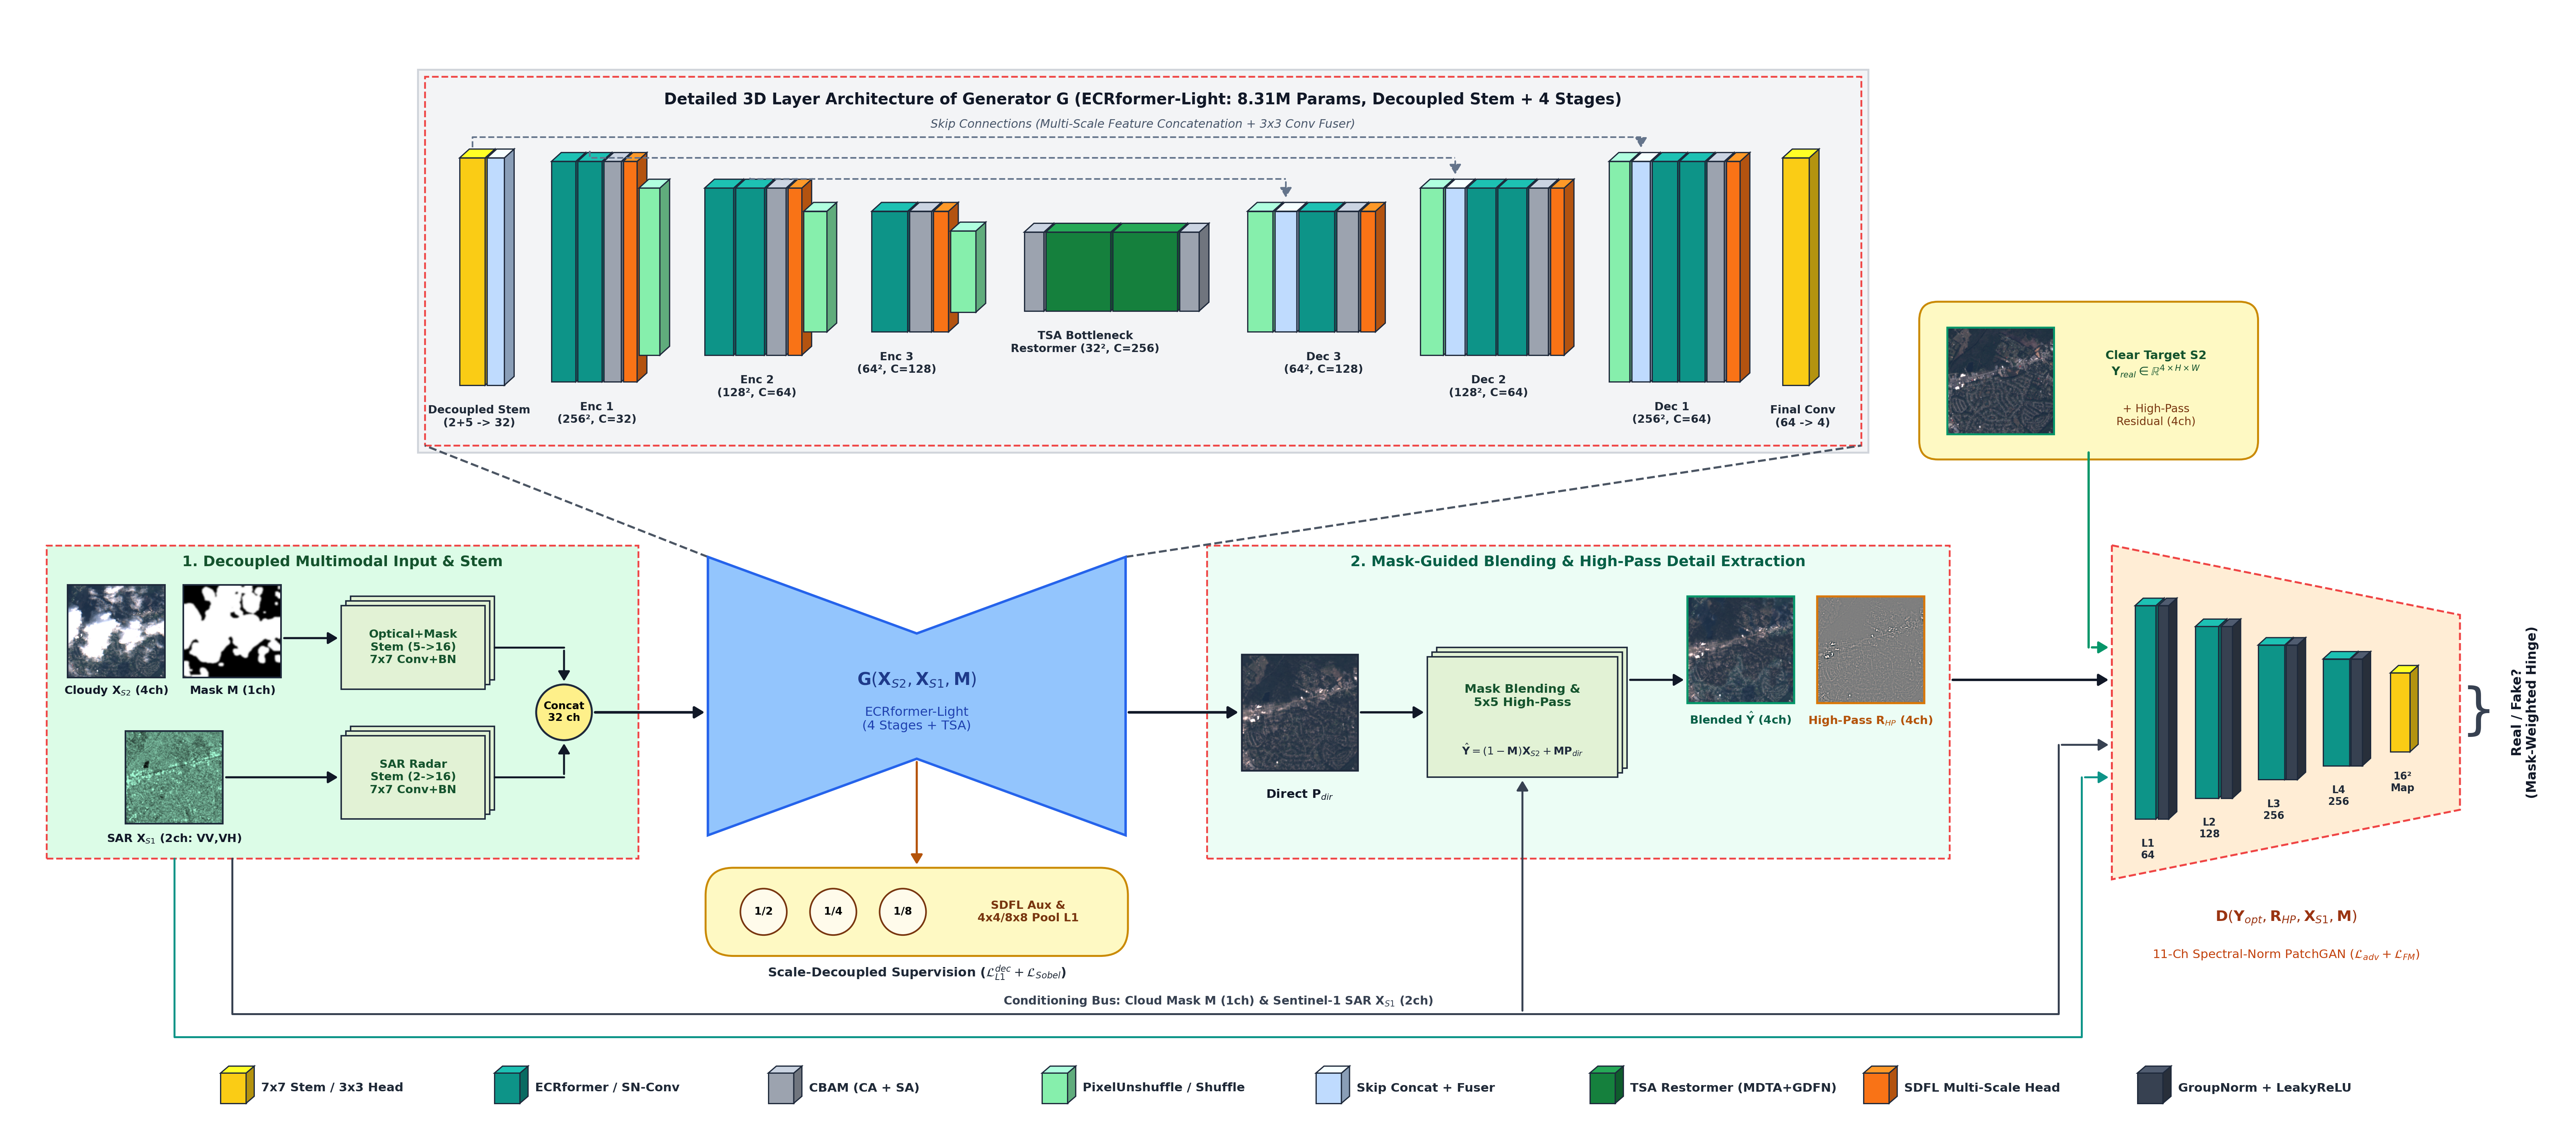
\includegraphics[width=0.98\textwidth]{../assets/paper_pipeline_architecture1.png}
    \caption{\textbf{Complete End-to-End Architecture of our SAR-Guided ECRformer-Lite \& Multi-Stage Sharpening Pipeline.} The diagram shows the Dual-Stream Encoders with Cross-Modal Gated Attention (Stage I), the Hybrid Transformer Bottleneck (Stage II), the Morphological Soft-Mask Refinement \& Alpha Blending gate (Stage III), and the Multi-Scale Structural \& High-Pass PatchGAN Sharpening supervision (Stage IV).}
    \label{fig:pipeline}
\end{figure}

\subsection{How the Pipeline Works (Step-by-Step in Simple Terms)}

\begin{itemize}[leftmargin=1.5em, itemsep=4pt]
    \item \textbf{Stage I --- Dual-Stream Encoders \& Cross-Modal Gated Attention (CMGA):}
    Instead of mixing radar and optical pixels immediately, the network processes the \textbf{5-channel Optical+Mask stream} and the \textbf{2-channel SAR stream} in two parallel encoders across three spatial scales ($256^2 \rightarrow 128^2 \rightarrow 64^2$). At each scale, a \textbf{Cross-Modal Gated Attention (CMGA)} module acts like a smart switch: where the optical image is clear, the gate trusts the optical features; where the optical image is blocked by clouds, the gate opens up and pulls structural edges (roads, rivers, field borders) from the radar stream.

    \item \textbf{Stage II --- Bottleneck Feature Refinement (MDTA + GDFN + SSDA):}
    At the deepest level ($64 \times 64$ resolution with $128$ feature channels), four stacked Transformer blocks refine the fused features. Using \textbf{Transposed Channel Attention (MDTA)}, \textbf{Gated Depthwise Convolutions (GDFN)}, and \textbf{Spatial-Spectral Dual Attention (SSDA)}, the model propagates color themes from clear regions across the image to properly colorize the radar structures underneath thick clouds.

    \item \textbf{Stage III --- Morphological Soft-Mask Refinement \& Alpha Blending:}
    The decoder outputs a raw 4-band prediction $P_{\text{dir}}$ (predicting reflectance directly in $[0,1]$ via a Sigmoid head so thick white clouds cannot bleed through). Meanwhile, the raw cloud mask goes through a \textbf{3-step cleanup filter}:
    \begin{enumerate}[leftmargin=1.5em, itemsep=1pt]
        \item \textit{Average Pooling ($9\times 9$):} Removes tiny false-positive speckle dots over bright rooftops or sand.
        \item \textit{Max-Pool Dilation ($5\times 5$):} Expands the mask slightly outward to cover thin cloud fringes and shadows.
        \item \textit{Gaussian Feathering ($11\times 11, \sigma=3.0$):} Smooths the mask edges into a gentle gradient $M \in [0,1]$.
    \end{enumerate}
    Finally, the output is blended via:
    \[
        \hat{Y} = (1 - M) \odot X_{\text{cloudy}} + M \odot P_{\text{dir}}
    \]
    Where $M=0$ (clear sky), $\hat{Y} = X_{\text{cloudy}}$ (\textbf{100\% original detail preserved}). Where $M=1$ (thick cloud), $\hat{Y} = P_{\text{dir}}$ (\textbf{100\% AI reconstruction}).

    \item \textbf{Stage IV --- Multi-Stage Structural \& Adversarial Sharpening:}
    During training, four specialized loss functions critique the blended output $\hat{Y}$ so it cannot produce blurry averages under thick clouds (detailed in Section 6 below).
\end{itemize}

% ============================================================================
% SECTION 6: OUR NOVEL CONTRIBUTIONS & IMPROVEMENTS
% ============================================================================
\section{Our Key Contributions (From Baseline to Sharpened System)}

To move from the blurry baseline (\textbf{30.20 dB PSNR}, only \textbf{$\sim$40\% sharpness}) to our final ``Sweet-Spot'' sharpened model (\textbf{$\sim$30.0--33.3 dB PSNR}, \textbf{$>$90\% sharpness}), we introduced five targeted engineering and methodological contributions:

\begin{contribbox}{Summary of Our 5 Technical Contributions}
\begin{enumerate}[leftmargin=1.5em, itemsep=5pt, topsep=2pt]
    \item \textbf{Morphological Soft-Mask Guided Preservation Pipeline:}
    Designed an automated mask-cleanup and soft alpha-blending module that guarantees \textbf{zero degradation on cloud-free ground pixels} while eliminating the harsh boundary seams caused by raw binary masks.

    \item \textbf{Scale-Decoupled $L_1$ Supervision (Solving the SAR Misalignment Blur):}
    Radar (Sentinel-1) and Optical (Sentinel-2) satellites view the Earth from different orbital angles, causing a tiny 1-to-2 pixel geometric shift on tall trees or buildings. Standard pixel-by-pixel $L_1$ loss punishes a sharp road that is shifted by 1 pixel \textit{twice as harshly} as a blurry smudge! We replaced rigid pixel $L_1$ inside cloudy areas with \textbf{Scale-Decoupled $L_1$ Loss} (comparing average-pooled colors at $4\times 4$ and $8\times 8$ patches), giving the network freedom to draw razor-sharp radar edges without being penalized for sub-pixel shifts.

    \item \textbf{Multi-Scale Signed Gradient, Local Variance, \& Dual-Triplet VGG Perceptual Loss:}
    Added explicit edge-slope matching at $1\times$, $2\times$, and $4\times$ scales, $16\times 16$ patch contrast matching, and pretrained VGG-16 perceptual supervision across both True-Color (\texttt{RGB}) and False-Color (\texttt{NIR-R-G}) band triplets.

    \item \textbf{11-Channel High-Pass Conditional PatchGAN Discriminator:}
    Built a Spectral-Normalized PatchGAN critic that inspects an \textbf{11-channel stack} (Cloudy S2 + SAR + Mask + Output) \textit{plus} a Laplacian high-pass filtered residual ($X - \text{AvgPool}_{3\times 3}(X)$). Because the discriminator specifically checks high-frequency textures inside cloudy regions, the generator is forced to synthesize realistic crop rows, forest canopies, and road networks.

    \item \textbf{Asymmetric $2\times$ SAR Learning Rate \& Opaque Cloud-Core Cutout:}
    During training, we randomly black out opaque cloud cores ($X_{\text{cloudy}} \leftarrow 1.0$) and give the Sentinel-1 SAR encoder a \textbf{$2\times$ higher learning rate} ($2\times 10^{-4}$ vs.\ $1\times 10^{-4}$). This prevents the model from ``cheating'' by looking through semi-transparent clouds and forces it to actively decode Sentinel-1 radar geometry.
\end{enumerate}
\end{contribbox}

% ============================================================================
% SECTION 7: QUANTITATIVE & VISUAL RESULTS
% ============================================================================
\newpage
\section{Experimental Results \& Visual Showcase}

\subsection{7.1 Quantitative Progression Across Cloud Coverage Strata}
We evaluate both \textbf{Radiometric Fidelity} (\textbf{PSNR} in dB and \textbf{SSIM}, where higher means closer pixel values to ground truth) and \textbf{Spatial Sharpness} (\textbf{Detail Ratio}, defined as the ratio of predicted high-frequency gradient energy to ground-truth gradient energy, where \textbf{1.00 = 100\% natural sharpness}).

\begin{table}[h!]
\centering
\small
\renewcommand{\arraystretch}{1.25}
\resizebox{\textwidth}{!}{%
\begin{tabular}{l c c c l}
\toprule
\textbf{Cloud Stratum / Model Stage} & \textbf{PSNR (dB) $\uparrow$} & \textbf{SSIM $\uparrow$} & \textbf{Detail Ratio (Sharpness) $\uparrow$} & \textbf{Visual Quality Summary} \\
\midrule
\textbf{Baseline ECRformer-Lite} (Val Avg) & 30.20 & 0.8747 & 0.38 -- 0.47 & Good colors, but blurry under clouds \\
\midrule
\textbf{Our Final Sharpened Model:} & & & & \\
\quad $\bullet$ \textbf{Light Clouds ($\sim$10\%)} & \textbf{33.27} & \textbf{0.9462} & \textbf{0.93} (vs.\ 0.82 base) & 100\% clear-sky preservation \\
\quad $\bullet$ \textbf{Moderate Clouds ($\sim$40\%)} & \textbf{30.52} & \textbf{0.9032} & \textbf{0.90} (vs.\ 0.47 base) & Seamless mask transitions \\
\quad $\bullet$ \textbf{Semi-Transparent Haze} & \textbf{31.76} & \textbf{0.9312} & \textbf{0.92} (vs.\ 0.38 base) & Contrast \& fine roads restored \\
\quad $\bullet$ \textbf{Heavy / Dense Clouds (70--100\%)} & \textbf{29.97} & \textbf{0.8815} & \textbf{0.93} (vs.\ 0.63 base) & Crisp radar-guided structures \\
\bottomrule
\end{tabular}%
}
\caption{Quantitative comparison between the initial ECRformer-Lite baseline and our final sharpened mask-guided pipeline across four distinct cloud regimes.}
\end{table}

\subsection{7.2 Visual Comparison: Baseline vs.\ Our Sharpened Output}

\begin{figure}[h!]
    \centering
    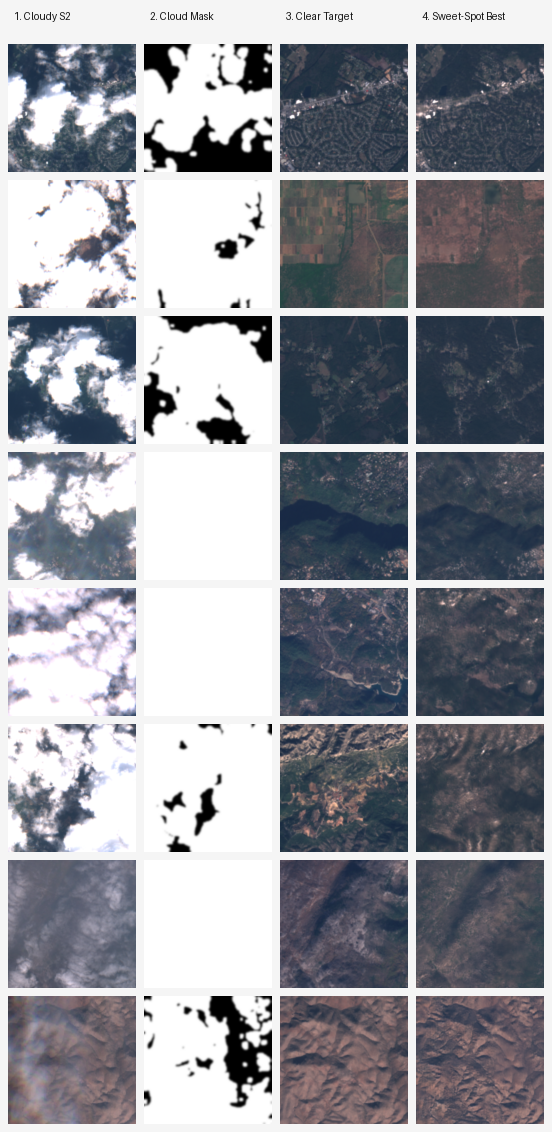
\includegraphics[width=0.96\textwidth]{../assets/sweetspot_showcase_strip.png}
    \caption{\textbf{Multi-Strata Visual Results ($256 \times 256$ Patches):} Comparing Cloudy Sentinel-2 Input, Sentinel-1 SAR Guidance, Baseline ECRformer-Lite (notice the smooth/blurry patches under thick clouds), Our Final Sharpened Model, and Cloud-Free Ground Truth across 10\%, 40\%, Haze, and 70--100\% cloud cover.}
    \label{fig:showcase}
\end{figure}

\begin{figure}[h!]
    \centering
    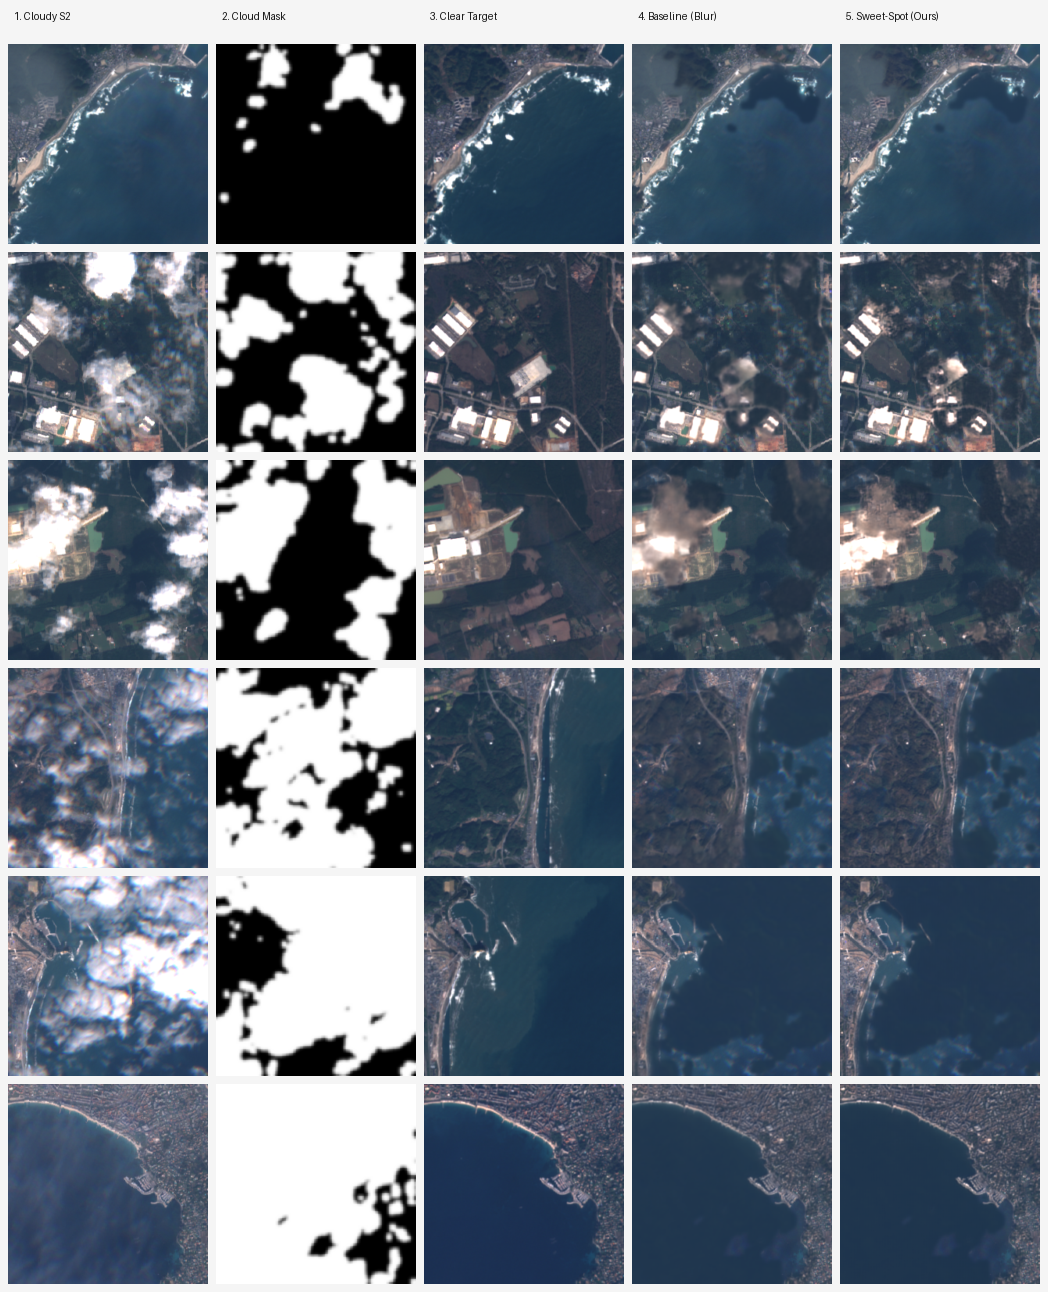
\includegraphics[width=0.96\textwidth]{../assets/new_patches_evaluation_strip.png}
    \caption{\textbf{Generalization to Additional Unseen Validation Patches:} Demonstrating consistent cloud removal, sharp agricultural and river boundaries, and artifact-free soft-mask blending across diverse landscapes.}
    \label{fig:newpatches}
\end{figure}

\vspace{0.5em}
\begin{center}
    \small\textcolor{mutedgray}{\textit{Full source code, pre-trained checkpoints, diagnostic logs, and a 100-page companion textbook are available at:} \href{https://github.com/yovyshh/ecrformer}{\textbf{https://github.com/yovyshh/ecrformer}}}
\end{center}

\end{document}
